%TOASK
%---------------------------------------------------------------------
%   documentclass
%---------------------------------------------------------------------
\documentclass[]{beamer}
% Class options include: notes, notesonly, handout, trans,
%                        hidesubsections, shadesubsections,
%                        inrow, blue, red, grey, brown

%---------------------------------------------------------------------
%   packages
%---------------------------------------------------------------------
% Theme for beamer presentation.
\usepackage{beamerthemesplit}
% Other themes include: beamerthemebars, beamerthemelined,
%                       beamerthemetree, beamerthemetreebars
\usepackage[english]{babel}
\usepackage[enc=cp1250]{hrlatex}
\usepackage[T1]{fontenc} %pekne makcene
\usepackage{lmodern} %spolu s T1 smooth font!
\usepackage{tikz}
\usepackage{cite} %bibtex
\usepackage[numbers]{natbib}
\usepackage{color} %for \textcolor{declared-color}{text}
\usepackage{floatflt} %to have tables and text beside
\usepackage{colortbl} %for \rowcolor command
\usepackage{scalefnt} %for scale font
\usepackage{pifont} %for ticks (check symbols)
\usetikzlibrary{decorations.pathreplacing}

%---------------------------------------------------------------------
%   settings
%---------------------------------------------------------------------
\graphicspath{{./pics/}} %picture dir

\definecolor{tablehead}{RGB}{238,233,233} %nice smooth grey

\def\Tiny{ \font\Tinyfont = cmr10 at 3pt \relax  \Tinyfont}

\pgfrealjobname{presentation} % <-- NOTE: this needs to be the real document's basename
                        %     (else you'll only get an empty output file)

\newif\iffull
\fullfalse

\newif\iffinal % introduce a switch for draft vs. final document
\finaltrue % use this to compile the final document
\iffinal
  \newcommand{\inputTikZ}[1]{%
    \input{#1.tikz}%
  }
\else
  \newcommand{\inputTikZ}[1]{%
    \beginpgfgraphicnamed{#1-external}%
    \input{#1.tikz}%
    \endpgfgraphicnamed%
  }
\fi

%---------------------------------------------------------------------
%   environments
%---------------------------------------------------------------------
%\newcommand{\newblock}{}

\newcommand{\tick}{\ding{52}}
\newcommand{\cross}{\ding{55}}

%---------------------------------------------------------------------
%   theme
%---------------------------------------------------------------------
\usetheme{Darmstadt}
\usecolortheme{crane}

%---------------------------------------------------------------------
%   data
%---------------------------------------------------------------------
\title{\textbf{Oracles for timetable graphs}}
\subtitle{Or�kula pre grafy reprezentuj�ce cestovn� poriadky}
\author{\textbf{Franti�ek Hajnovi�}}
\institute{FMFI UK}
\date{\today}

%---------------------------------------------------------------------
%   document
%---------------------------------------------------------------------
\begin{document}

	%---------------------------------------------------------------------
	%   Title page
	%---------------------------------------------------------------------
	{
    \setbeamertemplate{background canvas}{
        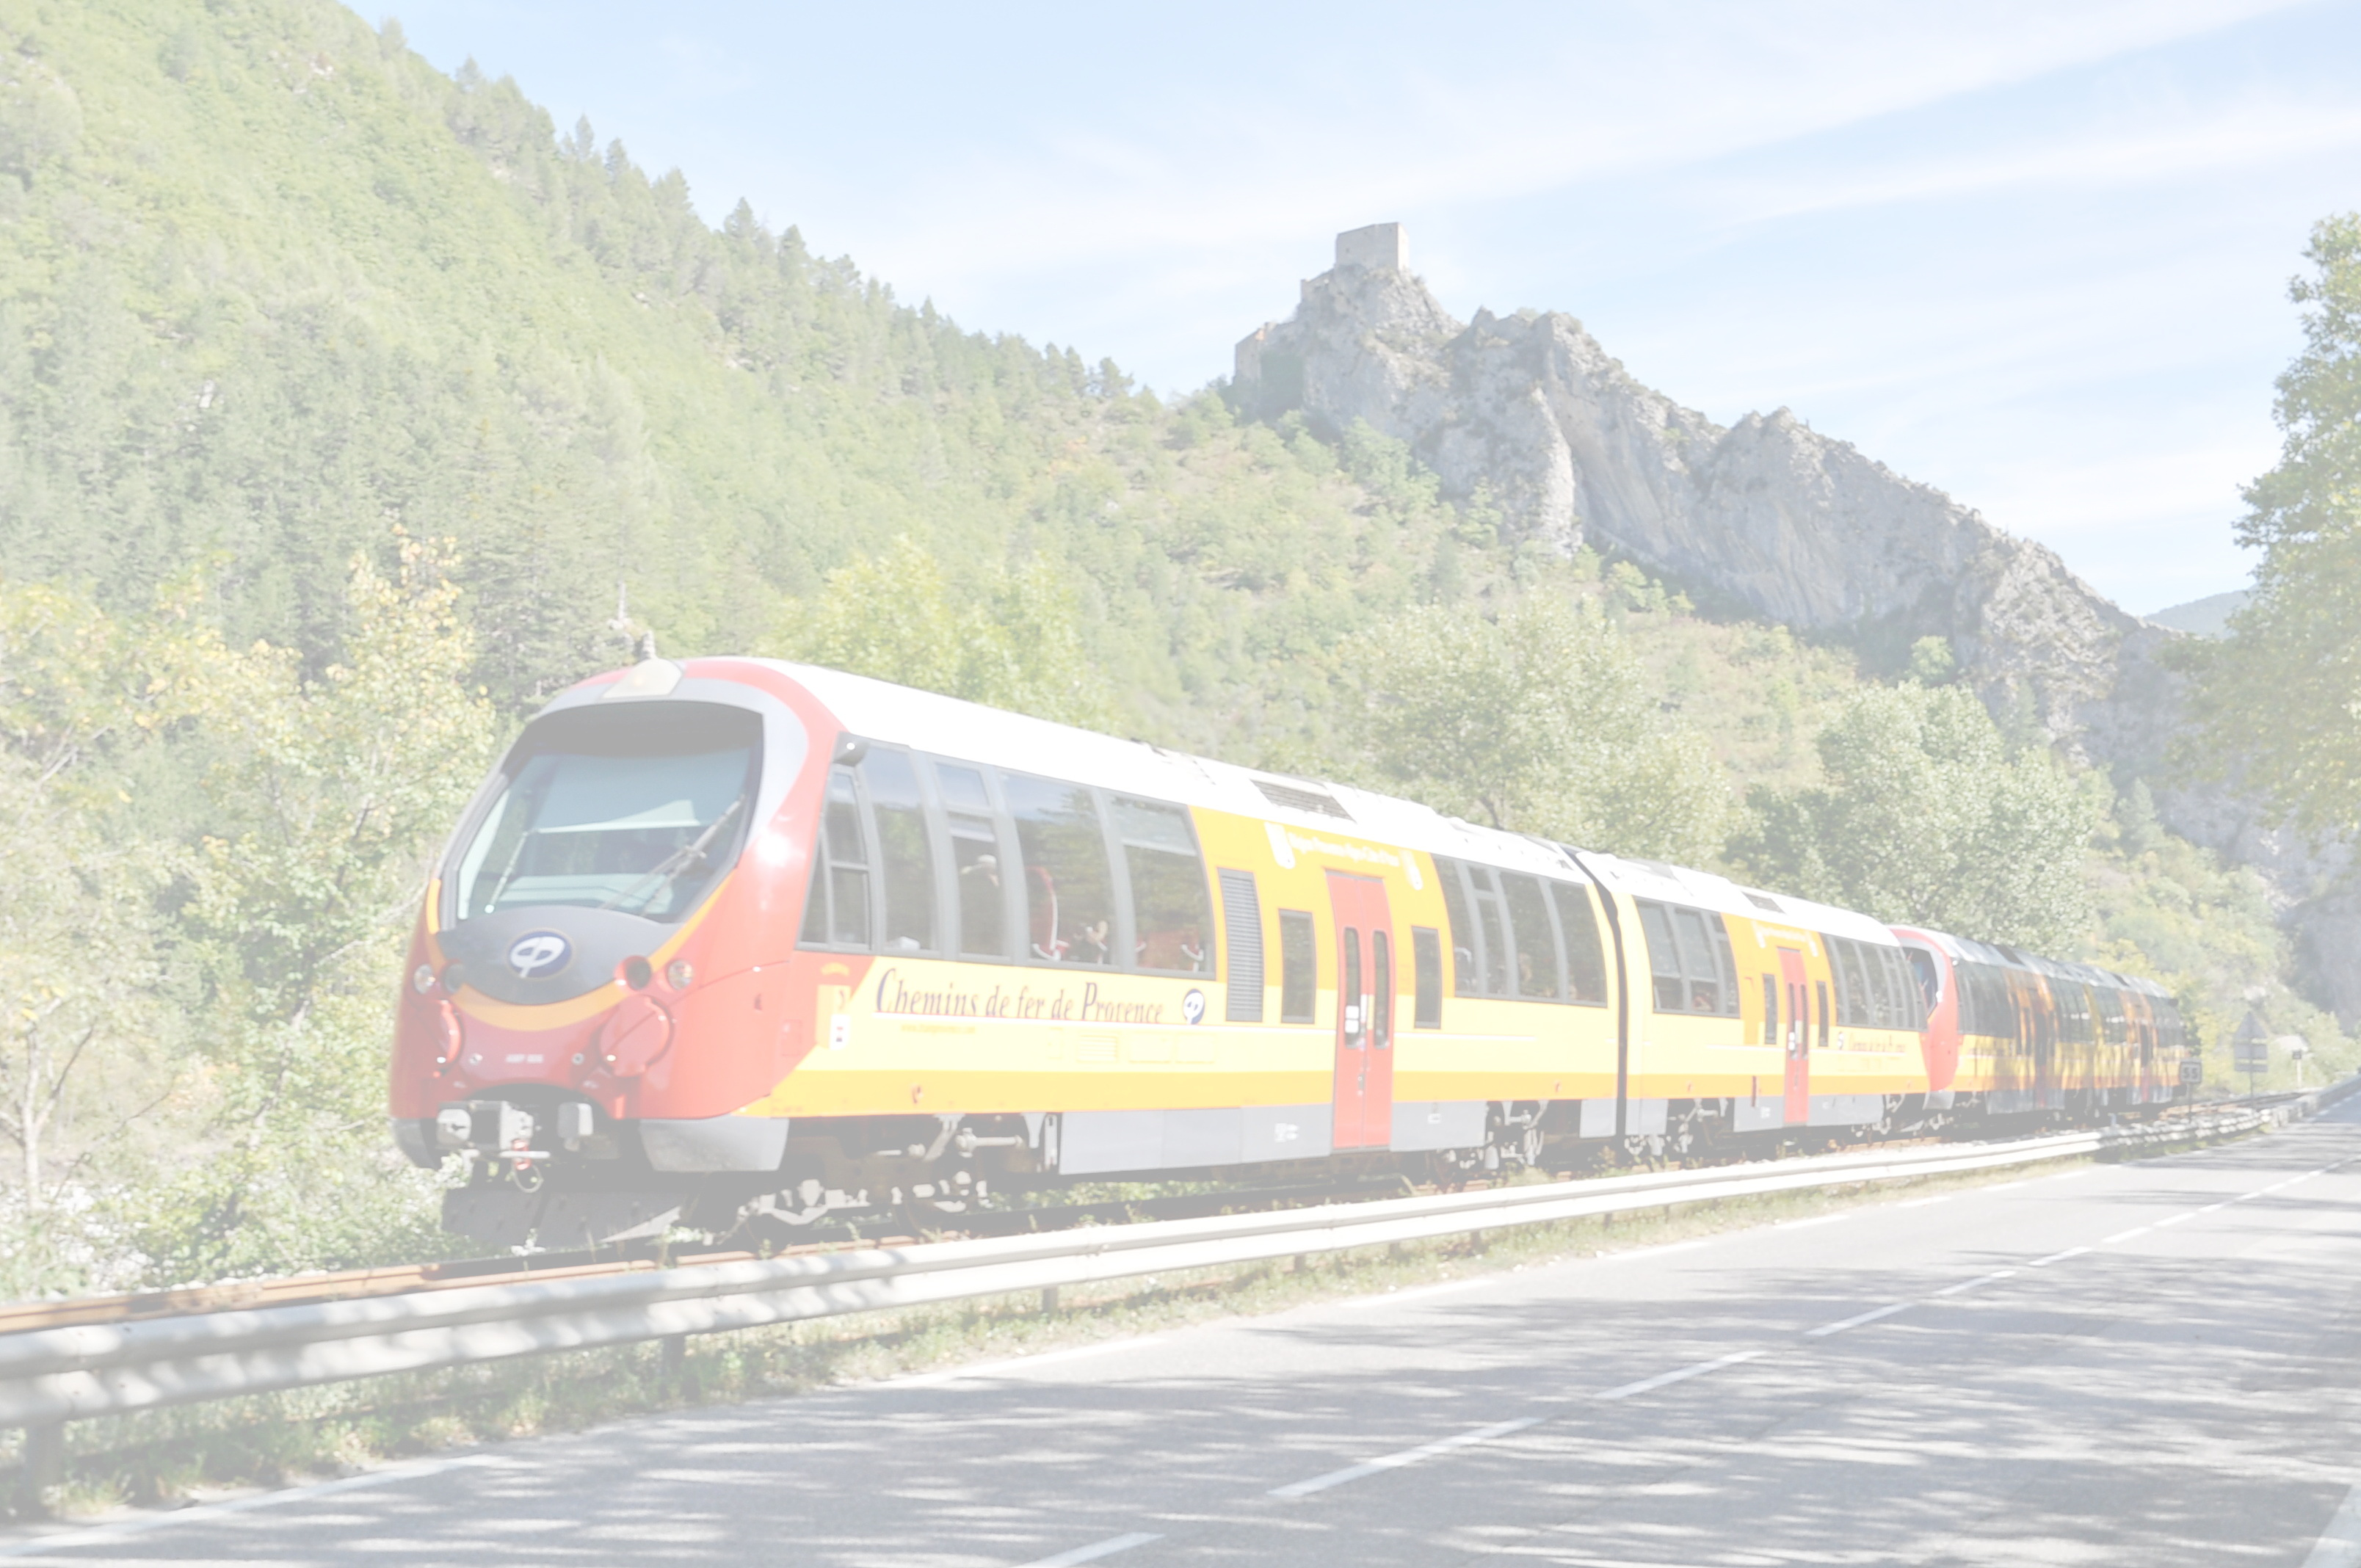
\includegraphics[height=\paperheight]{train.jpg}
    }
    \begin{frame}
        \titlepage
        \begin{center}
            Supervisor: \textit{doc. RNDr.} Rastislav Kr�lovi� \textit{PhD.}
        \end{center}
    \end{frame}
    }

	%---------------------------------------------------------------------
	%   Content
	%---------------------------------------------------------------------
    \begin{frame}
        \frametitle{Content}
        \tableofcontents
    \end{frame}

	%---------------------------------------------------------------------
	%   Introduction
	%---------------------------------------------------------------------
    \setbeamercolor{frametitle}{fg=red!80!black}
    \section{Introduction}
    \begin{frame}
        \frametitle{Introduction}
        \begin{center}
            \textcolor{red!80!black}{\textbf{Introduction}}
        \end{center}
    \end{frame}
    \setbeamercolor{frametitle}{fg=black!70}

		%---------------------------------------------------------------------
		%   What is it about?
		%---------------------------------------------------------------------
	    \begin{frame}
	        \frametitle{What is it about?}
	        \begin{itemize}
	            \item \textbf{Earliest arrival problem} (EAP) given a timetable
	            \begin{itemize}
	            	\item EA only
	            	\item Connection also
	            \end{itemize}
	        \end{itemize}
	        \begin{figure}[h!]
				\scriptsize
                \begin{center}
					\inputTikZ{./tikzpics/connection}
                \end{center}
                \caption{\textbf{Connection}, \textbf{elementary connection} and \textbf{earliest arrival}}
            \end{figure}
	    \end{frame}

		%---------------------------------------------------------------------
        %   Motivation
        %---------------------------------------------------------------------
        \subsection{Motivation \& usage}
        \begin{frame}
            \frametitle{Motivation \& usage}
            \begin{itemize}
                \item Timetable search engines (\emph{cp.sk, imhd.sk}...)
	            \item Bigger scale (e.g. Europe-wide)
            \end{itemize}
            \begin{figure}[h!]
	            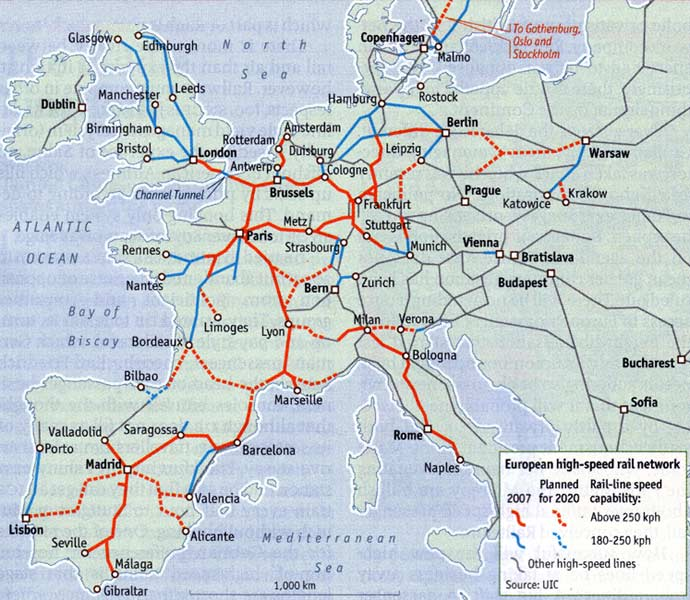
\includegraphics[height=1.65in]{europerails.jpg}
        	\end{figure}
        \end{frame}
        
        %---------------------------------------------------------------------
        %   TT and TE graph
        %---------------------------------------------------------------------
		\subsection{Definitions}
        \begin{frame}
            \frametitle{Timetable and Time-expanded graph~\cite{timetablemodelsalgs07}}        
	        \begin{columns}[c]
            \column{2.5in}
				\uncover<1->{\begin{table}{
	                \scriptsize
	                \begin{tabular}{c|c|c|c}
	                %legend
	                    \hline
	                    \rowcolor{tablehead}
	                    \multicolumn{2}{>{\columncolor{tablehead}}c|}{\textbf{Place}} & \multicolumn{2}{>{\columncolor{tablehead}}c}{\textbf{Time}} \\
						\hline
	                    \rowcolor{tablehead}
	                    \textbf{From} & \textbf{To} & \textbf{Departure} & \textbf{Arrival} \\
	                %data
						\hline
						\textcolor{orange}{A} & \textcolor{orange}{B} & 10:00 & 10:45 \\
						\textcolor{orange}{B} & \textcolor{orange}{C} & 11:00 & 11:30 \\
						\textcolor{orange}{B} & \textcolor{orange}{C} & 11:30 & 12:10 \\
						\textcolor{orange}{B} & \textcolor{orange}{A} & 11:20 & 12:30 \\
						\textcolor{orange}{C} & \textcolor{orange}{A} & 11:45 & 12:15 \\
					\end{tabular}}
					\caption{\textbf{Timetable} - a set of \textcolor{red}{\textbf{elementary connections}} (between pairs of \textbf{\textcolor{orange}{cities}})}
	            	\normalsize
				\end{table}}
            \column{2.5in}
            	\uncover<2->{\begin{figure}[h!]
					\scriptsize
	                \begin{center}
						\inputTikZ{./tikzpics/te}
	                \end{center}
                    \caption{\textbf{Time-expanded graph} - \textit{\textcolor{red}{connection}} and \textit{\textcolor{olive}{waiting}} edges. Nodes are called \textbf{\textcolor{blue}{events}}}
                \end{figure}}
			\end{columns}
			\begin{itemize}
				\item<3-> \textbf{Height} - $max_{c \in cities}\{\# \; of \; events \; in \; c\}$
			\end{itemize}
		\end{frame}
		
		%---------------------------------------------------------------------
        %   TT and TD graph
        %---------------------------------------------------------------------
        \begin{frame}
            \frametitle{Time-dependent graph~\cite{timetablemodelsalgs07}}        
	        \begin{columns}[c]
            \column{2.5in}
				\uncover<1->{\begin{table}{
	                \tiny
	                \begin{tabular}{c|c|c|c}
	                %legend
	                    \hline
	                    \rowcolor{tablehead}
	                    \multicolumn{2}{>{\columncolor{tablehead}}c|}{\textbf{Place}} & \multicolumn{2}{>{\columncolor{tablehead}}c}{\textbf{Time}} \\
						\hline
	                    \rowcolor{tablehead}
	                    \textbf{From} & \textbf{To} & \textbf{Departure} & \textbf{Arrival} \\
	                %data
						\hline
	                    \textcolor{orange}{A} & \textcolor{orange}{B} & 10:00 & 10:45 \\
						\textcolor{orange}{B} & \textcolor{orange}{C} & 11:00 & 11:30 \\
						\textcolor{orange}{B} & \textcolor{orange}{C} & 11:30 & 12:10 \\
						\textcolor{orange}{B} & \textcolor{orange}{A} & 11:20 & 12:30 \\
						\textcolor{orange}{C} & \textcolor{orange}{A} & 11:45 & 12:15 \\
					\end{tabular}}
					\caption{\textbf{Timetable} - a set of \textcolor{red}{\textbf{elementary connections}} (between pairs of \textbf{\textcolor{orange}{cities}})}
	            	\normalsize
				\end{table}}
				\uncover<2->{\begin{figure}[h!]
					\scriptsize
	                \begin{center}
						\inputTikZ{./tikzpics/td}
	                \end{center}
                    \caption{\textbf{Time-dependent graph}}
                \end{figure}}
            \column{2.5in}
                \uncover<3->{\begin{figure}[h!]
					\scriptsize
	                \begin{center}
						\inputTikZ{./tikzpics/tdpiece}
	                \end{center}
                    \caption{Piece-wise linear function}
                \end{figure}}
			\end{columns}
		\end{frame}
		
		%---------------------------------------------------------------------
        %   TT and UG graph
        %---------------------------------------------------------------------
        \begin{frame}
            \frametitle{Underlying graph}        
	        \begin{columns}[c]
            \column{2.5in}
				\begin{table}{
	                \scriptsize
	                \begin{tabular}{c|c|c|c}
	                %legend
	                    \hline
	                    \rowcolor{tablehead}
	                    \multicolumn{2}{>{\columncolor{tablehead}}c|}{\textbf{Place}} & \multicolumn{2}{>{\columncolor{tablehead}}c}{\textbf{Time}} \\
						\hline
	                    \rowcolor{tablehead}
	                    \textbf{From} & \textbf{To} & \textbf{Departure} & \textbf{Arrival} \\
	                %data
						\hline
	                    \textcolor{orange}{A} & \textcolor{orange}{B} & 10:00 & 10:45 \\
						\textcolor{orange}{B} & \textcolor{orange}{C} & 11:00 & 11:30 \\
						\textcolor{orange}{B} & \textcolor{orange}{C} & 11:30 & 12:10 \\
						\textcolor{orange}{B} & \textcolor{orange}{A} & 11:20 & 12:30 \\
						\textcolor{orange}{C} & \textcolor{orange}{A} & 11:45 & 12:15 \\
					\end{tabular}}
					\caption{\textbf{Timetable} - a set of \textcolor{red}{\textbf{elementary connections}} (between pairs of \textbf{\textcolor{orange}{cities}})}
	            	\normalsize
				\end{table}
            \column{2.5in}
            	\begin{figure}[h!]
					\scriptsize
	                \begin{center}
						\inputTikZ{./tikzpics/ug}
	                \end{center}
                    \caption{\textbf{Underlying graph}}
                \end{figure}
			\end{columns}
		\end{frame}
		
        %---------------------------------------------------------------------
        %   Oracles
        %---------------------------------------------------------------------
        \begin{frame}
            \frametitle{Oracle}
            \begin{columns}[c]
            \column{2.7in}
		        \begin{itemize}
	                \item<1-> Dijkstra's algorithm $\mathcal{O}(m + n \log n)$
	                \item<2-> Precompute information $\rightarrow$ \textbf{Oracle based method}
	                \begin{itemize}
		                \small
	                    \item \textit{Preprocessing time}
	                    \item \textit{Size}
	                    \item \textit{Query time}
	                    \item \textit{Stretch}
	                \end{itemize}
	            \end{itemize}    
            \column{2.3in}
				\uncover<2->{\begin{figure}[h]
					\scriptsize
                    \begin{center}
                    	\inputTikZ{./tikzpics/compromises}
                    \end{center}
					\caption{Compromises between parameters}
                \end{figure}}
            \end{columns}
            \uncover<2->{\begin{figure}[h!]
                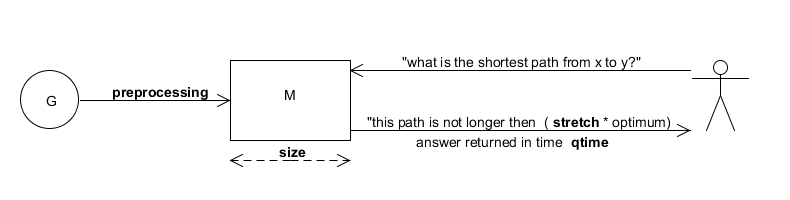
\includegraphics[height=0.9in]{dodiagram.png}
                \caption{Oracle based method}
            \end{figure}}
        \end{frame}       
      
		%---------------------------------------------------------------------
        %   Goals
        %---------------------------------------------------------------------
        \subsection{Goals}
        \begin{frame}
            \frametitle{Goals}
			\begin{columns}[c]
            \column{2.7in}
		        \begin{itemize}
	                \item Devise methods to tackle EAP
		            \item Analyse properties of timetables
	            \end{itemize}
            \column{2.3in}
	            \uncover<2->{\begin{figure}[h!]
	                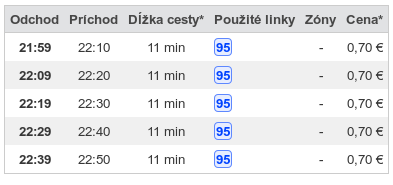
\includegraphics[height=0.9in]{redundancy.png}
	                \caption{Exploit redundancy in timetables?}
	            \end{figure}}
	        \end{columns}
        \end{frame}  
            
	%---------------------------------------------------------------------
	%   Data 
	%---------------------------------------------------------------------
    \setbeamercolor{frametitle}{fg=red!80!black}
    \section{Data}
    \begin{frame}
        \frametitle{Data}
        \begin{center}
            \textcolor{red!80!black}{\textbf{Data}}
        \end{center}
    \end{frame}
    \setbeamercolor{frametitle}{fg=black!70}
    
	    %---------------------------------------------------------------------
        %   Data
        %---------------------------------------------------------------------
        \begin{frame}
            \frametitle{Data}
			\begin{table}{
                \scriptsize
                \begin{tabular}{c|c|c|c|c|c}
                %legend
                    \hline
                    \rowcolor{tablehead}
                    \textbf{Name} & \textbf{Description} & \textbf{El. conns.} & \textbf{Cities} & \textbf{Time range} & \textbf{Height ($h$)} \\
                %data
					\hline
					air01 & domestic flights (US) & 592767 & 250 & 1 month & 24374 \\
					cpru & regional bus (SVK) & 10011 & 250 & 1 day & 239 \\
					cpza & regional bus (SVK) & 15776 & 250 & 1 day & 370 \\
					montr & public transport (Montreal) & 7118 & 211 & 1 day & 363 \\
					zsr & country-wide rails (SVK) & 931647 & 233 & 1 year & 59928 \\
				\end{tabular}}
				\caption{Data - timetable properties}
            	\normalsize
			\end{table}
        \end{frame}

		%---------------------------------------------------------------------
        %   Data
        %---------------------------------------------------------------------
        \begin{frame}
            \frametitle{Data properties}
			\begin{table}{
                \scriptsize
                \begin{tabular}{c|c|c|c|c|c}
                %legend
                    \hline
                    \rowcolor{tablehead}
                    \textbf{Name} & \textbf{Arcs} & \textbf{Avg/Max deg.} & \textbf{Avg/Max SP} & \textbf{Max str. comp.} & \textbf{Avg betw.} \\
                %data
					\hline
					air01 & 4542 & 18.2/166 & 196.4/838 & 250 & 0.028 \\
					cpru & 779 & 3.2/17 & 20.2/95 & 250 & 0.083 \\
					cpza & 688 & 2.8/23 & 36.2/108 & 218 & 0.12 \\
					montr & 339 & 1.6/5 & 43.5/135 & 209 & 0.17 \\
					zsr & 588 & 2.5/12 & 169.7/450 & 225 & 0.11 \\
				\end{tabular}}
				\caption{Data - underlying graphs properties}
            	\normalsize
			\end{table}
        \end{frame}
                
	%---------------------------------------------------------------------
	%   USPs 
	%---------------------------------------------------------------------
    \setbeamercolor{frametitle}{fg=red!80!black}
    \section{Underlying shortest paths}
    \begin{frame}
        \frametitle{Underlying shortest paths}
        \begin{center}
            \textcolor{red!80!black}{\textbf{Underlying shortest paths}}
        \end{center}
        
    \end{frame}
    \setbeamercolor{frametitle}{fg=black!70}
    
	    %---------------------------------------------------------------------
        %   Idea
        %---------------------------------------------------------------------
        \begin{frame}
            \frametitle{Idea}
			\begin{itemize}
                \item \textit{``Usually we go through the same sequence of cities''}
            \end{itemize}
            \begin{columns}[c]
            \column{2.3in}
	            \begin{figure}[h]
					\scriptsize
	                \begin{center}
	                    \inputTikZ{./tikzpics/usp}
	                \end{center}
				\caption{\textbf{Underlying shortest path}}
	            \end{figure}
	            \begin{itemize}
	                \item<2-> \textbf{Overtaking} causes problems, but can be easily removed
	            \end{itemize}
	        \column{2.7in}
	            \uncover<2->{\begin{table}{
	                \scriptsize
	                \begin{tabular}{c|c}
	                %legend
	                    \hline
	                    \rowcolor{tablehead}
	                    \textbf{Name} & \textbf{Overtaken edges (\%)} \\
	                %data
						\hline
						air01 & 1\% \\
						cpru & 2\% \\
						cpza & 2\% \\
						montr & 1\% \\
						zsr & 0\% \\
					\end{tabular}}
					\caption{Data - underlying graphs properties}
	            	\normalsize
				\end{table}}
			\end{columns}
        \end{frame}
        
        %---------------------------------------------------------------------
        %   USP-OR
        %---------------------------------------------------------------------
        \subsection{USP-OR}
        \begin{frame}
            \frametitle{USP-OR}
            \begin{columns}[c]
            \column{2.9in}
				\begin{itemize}
					\item<1-> Pre-compute all connections - space $\mathcal{O}(h \; n^{3})$
					\begin{itemize}
	                	\item height $h \gg n$ 
	                \end{itemize}
	                \item<2-> Pre-compute all USPs - space $\mathcal{O}(\tau \; n^{3})$
	                \begin{itemize}
	                	\item Exact answers, $\mathcal{O}(\tau \; n)$ query time
	                	\item Preprocessing $\mathcal{O}((hn)^{3})$
	                	\item How big is $\tau$?
	                	\item<4-> Space too big anyway
	                \end{itemize}
	            \end{itemize}
	        \column{2.1in}
	        	\uncover<3->{\begin{table}{
	                \scriptsize
	                \begin{tabular}{c|c|c}
	                %legend
	                    \hline
	                    \rowcolor{tablehead}
	                    \textbf{Name} & \textbf{avg $\tau_{A, B}$} & \textbf{max $\tau_{A, B}$} \\
	                %data
						\hline
						air01 & 18.3 & 126 \\
						cpru & 10.25 & 53 \\
						cpza & 5.87 & 45 \\
						montr & 4.09 & 30 \\
						zsr & 8.9 & 85 \\
					\end{tabular}}
					\caption{$\tau_{A, B}$ - number of USPs between $A$ and $B$}
	            	\normalsize
				\end{table}}
	        \end{columns}
        \end{frame}  	
        
        %---------------------------------------------------------------------
        %   USP-OR-A
        %---------------------------------------------------------------------
        \subsection{USP-OR-A}
        \begin{frame}
            \frametitle{USP-OR-A}
			\begin{itemize}
				\item \textbf{Access nodes} - set $A$ of cities in \textit{UG}
				\begin{itemize}
					\item Size $|Acc| = \mathcal{O}(\sqrt{n})$
					\item Small node neighbourhoods $\forall v \; |neigh_{Acc}(v)| = \mathcal{O}(\sqrt{n})$
					\item Few local access nodes ($\forall v \; |Acc_{v}| = \mathcal{O}(f(n))$)
				\end{itemize}
				\begin{figure}[h]
					\scriptsize
	                \begin{center}
	                    \inputTikZ{./tikzpics/uspora}
	                \end{center}
				\caption{\textbf{Principle of access nodes}}
	            \end{figure}
	        \end{itemize}
        \end{frame} 
        
        %---------------------------------------------------------------------
        %   USP-OR-A
        %---------------------------------------------------------------------
        \begin{frame}
            \frametitle{USP-OR-A}
			\begin{itemize}
				\item Space $\mathcal{O}(\tau \; n^{2})$
				\item Query time $\mathcal{O}(\tau \; n \; f(n)^{2})$
				\begin{itemize}
					\item Search in neighbourhood can be Dijkstra
				\end{itemize}
				\item<2-> We may limit precomputed USPs
			\end{itemize}
			\uncover<2->{\begin{figure}[h]
				\scriptsize
                \begin{center}
                    \inputTikZ{./tikzpics/comprousp}
                \end{center}
				\caption{Decreasing $\tau$ to save resources}
            \end{figure}}
        \end{frame}
        
        %---------------------------------------------------------------------
        %   USP-OR-A
        %---------------------------------------------------------------------
        \begin{frame}
            \frametitle{USP-OR-A}
			\begin{itemize}
				\item Inspiration by TRANSIT algorithm \cite{transit06}
				\begin{itemize}
					\item 10 access nodes on average in road network
					\item<2-> Works thanks to low highway dimension
				\end{itemize}
			\end{itemize}
			\uncover<2->{\begin{table}{
                \scriptsize
                \begin{tabular}{c|c|c}
                %legend
                    \hline
                    \rowcolor{tablehead}
                    \textbf{Name} & \textbf{Apx. HD} & \textbf{normalized} \\
                %data
					\hline
					\textit{svk} & 18 & 0.072 \\
					air01 & 71 & 0.284 \\
					cpru & 59 & 0.236 \\
					cpza & 26 & 0.104 \\
					montr & 32 & 0.152 \\
					zsr & 21 & 0.090 \\
				\end{tabular}}
				\caption{Highway dimension for Slovak road network and UGs of the timetables}
            	\normalsize
			\end{table}}
        \end{frame}
        
        %---------------------------------------------------------------------
        %   Existing methods
        %---------------------------------------------------------------------
        \subsection{Existing methods}
        \begin{frame}
            \frametitle{Existing methods}
			\begin{itemize}
				\item \textbf{Time-dependent SHARC} \cite{sharc08}, \textbf{Time-dependent CH} \cite{timedepch09}
				\begin{itemize}
					\item Speed-ups of about 26 / 1500, respectively
					\item Meant for time-dependent routing in road networks
				\end{itemize}
				\item \textbf{Time-expanded approach} \cite{engtimeexp09}
				\begin{itemize}
					\item Speed-ups of about 56
					\item Remodelling unimportant stations
				\end{itemize}
			\end{itemize}
        \end{frame}
        
	%---------------------------------------------------------------------
	%   Neural networks 
	%---------------------------------------------------------------------
    \setbeamercolor{frametitle}{fg=red!80!black}
    \section{Neural networks}
    \begin{frame}
        \frametitle{Neural networks}
        \begin{center}
            \textcolor{red!80!black}{\textbf{Neural networks}}
        \end{center}
    \end{frame}
    \setbeamercolor{frametitle}{fg=black!70}              
      
        %---------------------------------------------------------------------
        %   Approaches
        %---------------------------------------------------------------------
        \begin{frame}
            \frametitle{Neural network approaches}
			\begin{itemize}
				\item Multi-layer perceptron, back propagation
				\item Input layer = \textcolor{blue}{events} + \textcolor{orange}{cities}. Output layer:
				\begin{enumerate}
					\item Arcs of UG $rightarrow$ USP
					\item Arcs of UG $rightarrow$ routing
					\item Earliest arrival value
				\end{enumerate}
			\end{itemize}
			\begin{figure}[h]
				\scriptsize
                \begin{center}
                    \inputTikZ{./tikzpics/neural}
                \end{center}
				\caption{Approach 1.)}
            \end{figure}
        \end{frame}  
        
        %---------------------------------------------------------------------
        %   Results
        %---------------------------------------------------------------------
        \begin{frame}
            \frametitle{Results}
			\begin{itemize}
				\item Tendency to remember USPs
				\item Long training times
			\end{itemize}            
			\begin{table}{
                \scriptsize
                \begin{tabular}{c|c|c|c}
                %legend
                    \hline
                    \rowcolor{tablehead}
                    \textbf{Name} & \textbf{Conn.} & \textbf{Found} & \textbf{Was optimum (\%)} \\
                %data
					\hline
					air01 & 931 & 573 & 18.7\% \\
					cpru & 481 & 281 & 48\% \\
					montr & 527 & 346 & 86.7\% \\
					zsr & 672 & 307 & 76.2\% \\
				\end{tabular}}
				\caption{Tests of a trained NN on timetables with 30 cities (approach 1.)}
            	\normalsize
			\end{table}
        \end{frame}
        
	%---------------------------------------------------------------------
	%   Application TTBlazer
	%---------------------------------------------------------------------
    \setbeamercolor{frametitle}{fg=red!80!black}
    \section{Application TTBlazer}
    \begin{frame}
        \frametitle{Application TTBlazer}
        \begin{center}
            \textcolor{red!80!black}{\textbf{Application TTBlazer}}
        \end{center}
    \end{frame}
    \setbeamercolor{frametitle}{fg=black!70}      
       
        %---------------------------------------------------------------------
        %   TTBlazer
        %---------------------------------------------------------------------
        \begin{frame}
            \frametitle{Timetable analyzer - TTBlazer}
			\begin{itemize}
				\item Works with UG, TE, TD, TT
				\item Analysis ($\tau$, HD, degrees...), oracles (USP-OR, Dijkstra...), modifications (remove overtaking...), generation (subgraphs, TT $\rightarrow$ TD ...)
				\item Running \& evaluating tests
				\item Easily extendible
			\end{itemize}
			\begin{figure}[h!]
                
\includegraphics[height=0.6in]{ttblazer.png}
                \caption{It's \textit{blazing} fast!}
            \end{figure}
        \end{frame}	
    
    %---------------------------------------------------------------------
	%   Conclusion
	%---------------------------------------------------------------------
    \setbeamercolor{frametitle}{fg=red!80!black}
    \section{Conclusion}
    \begin{frame}
        \frametitle{Conclusion}
        \begin{center}
            \textcolor{red!80!black}{\textbf{Conclusion}}
        \end{center}
    \end{frame}
    \setbeamercolor{frametitle}{fg=black!70}
    
    	%---------------------------------------------------------------------
        %   Conclusion
        %---------------------------------------------------------------------
        \subsection{Conclusion}
        \begin{frame}
            \frametitle{Conclusion}
			\begin{itemize}
				\item Trying out novel approaches to solving EAP in timetables
				\begin{itemize}
					\item \textit{USP-OR}: Exact and quick answers but high space and time preprocessing
					\item \textit{NN}: Problem too challenging for NN/try different types of network
				\end{itemize}
				\item Analysis of \textbf{various} real-world timetables
				\begin{itemize}
					\item Better insight on properties of timetables
				\end{itemize}
				\item Useful and easily extendible application
			\end{itemize}
        \end{frame}
        
        %---------------------------------------------------------------------
        %   TTBlazer
        %---------------------------------------------------------------------
        \subsection{To-do}
        \begin{frame}
            \frametitle{To-do}
            \begin{columns}[c]
            \column{2.9in}
				\begin{itemize}
					\item Find a good access node set
					\item Reduce the space complexity further
					\item Train and test properly neural network oracles
				\end{itemize}
			\column{2.1in}
				\begin{figure}[h!]
	                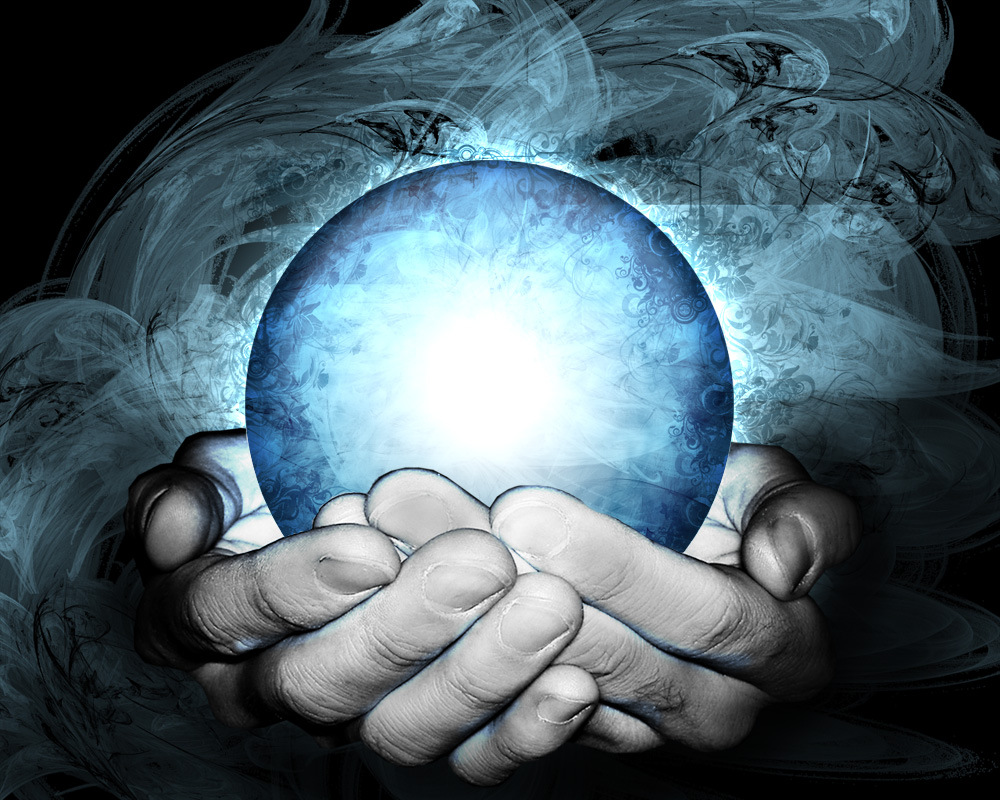
\includegraphics[height=1in]{crystall.jpg}
	            \end{figure}
			\end{columns}
        \end{frame}
        
%---------------------------------------------------------------------
%   Bibliography
%---------------------------------------------------------------------
    \begin{frame}[allowframebreaks]
        \frametitle{Bibliography}
        \tiny
        \bibliographystyle{is-alpha}
        \bibliography{../bibl}
        %compile latex, bibtex, latex, latex
    \end{frame}

%---------------------------------------------------------------------
%   Thanks for the attention
%---------------------------------------------------------------------
	{
    \setbeamertemplate{background canvas}{
        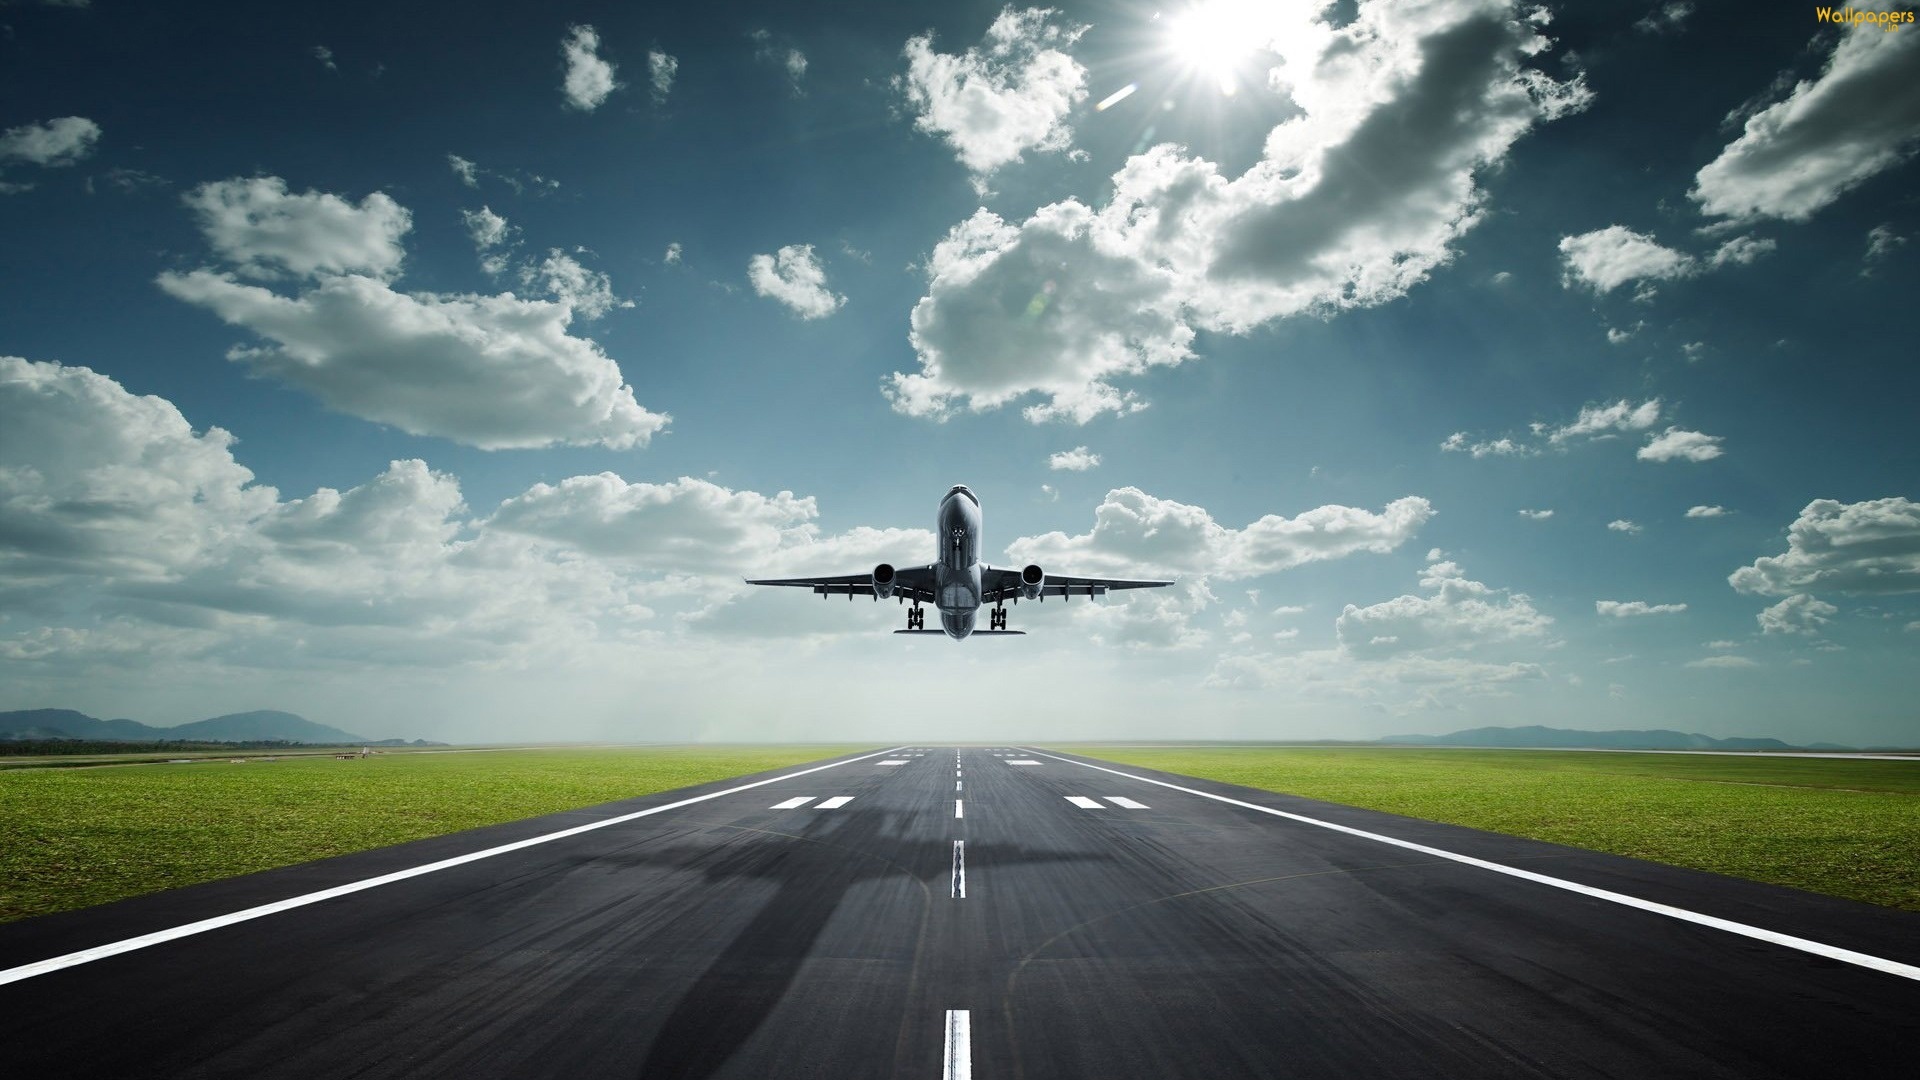
\includegraphics[height=\paperheight]{takeoff.jpg}
    }
    \begin{frame}
        \frametitle{Thank you for the attention}
        \begin{center}
        	\vskip 2cm
            \textbf{Thank you for the attention}
        \end{center}
    \end{frame}
    }

\end{document}
